
\documentclass{sig-alternate-05-2015}
% Pages are numbered in submission mode, and unnumbered in camera-ready
\usepackage{subfigure}
\usepackage{graphicx}
\usepackage{times}
\usepackage{epsfig}
%\usepackage{figure}

\usepackage{amsmath}
\usepackage{amssymb}
% Pages are numbered in submission mode, and unnumbered in camera-ready
\begin{document}
\setcopyright{acmcopyright}

%%%%%%%%% TITLE
\title{Title Here}

\author{
	% You can go ahead and credit any number of authors here,
	% e.g. one 'row of three' or two rows (consisting of one row of three
	% and a second row of one, two or three).
	%
	% The command \alignauthor (no curly braces needed) should
	% precede each author name, affiliation/snail-mail address and
	% e-mail address. Additionally, tag each line of
	% affiliation/address with \affaddr, and tag the
	% e-mail address with \email.
	%
	% 1st. author
	\alignauthor
	Yue Wu\titlenote\\
	\email{1600012704@pku.edu.cn}
}

\maketitle
%\thispagestyle{empty}


%%%%%%%%% ABSTRACT


%%%%%%%%% BODY TEXT
\section{Section one}

    \begin{figure}
		\begin{center}
		\subfigure{
		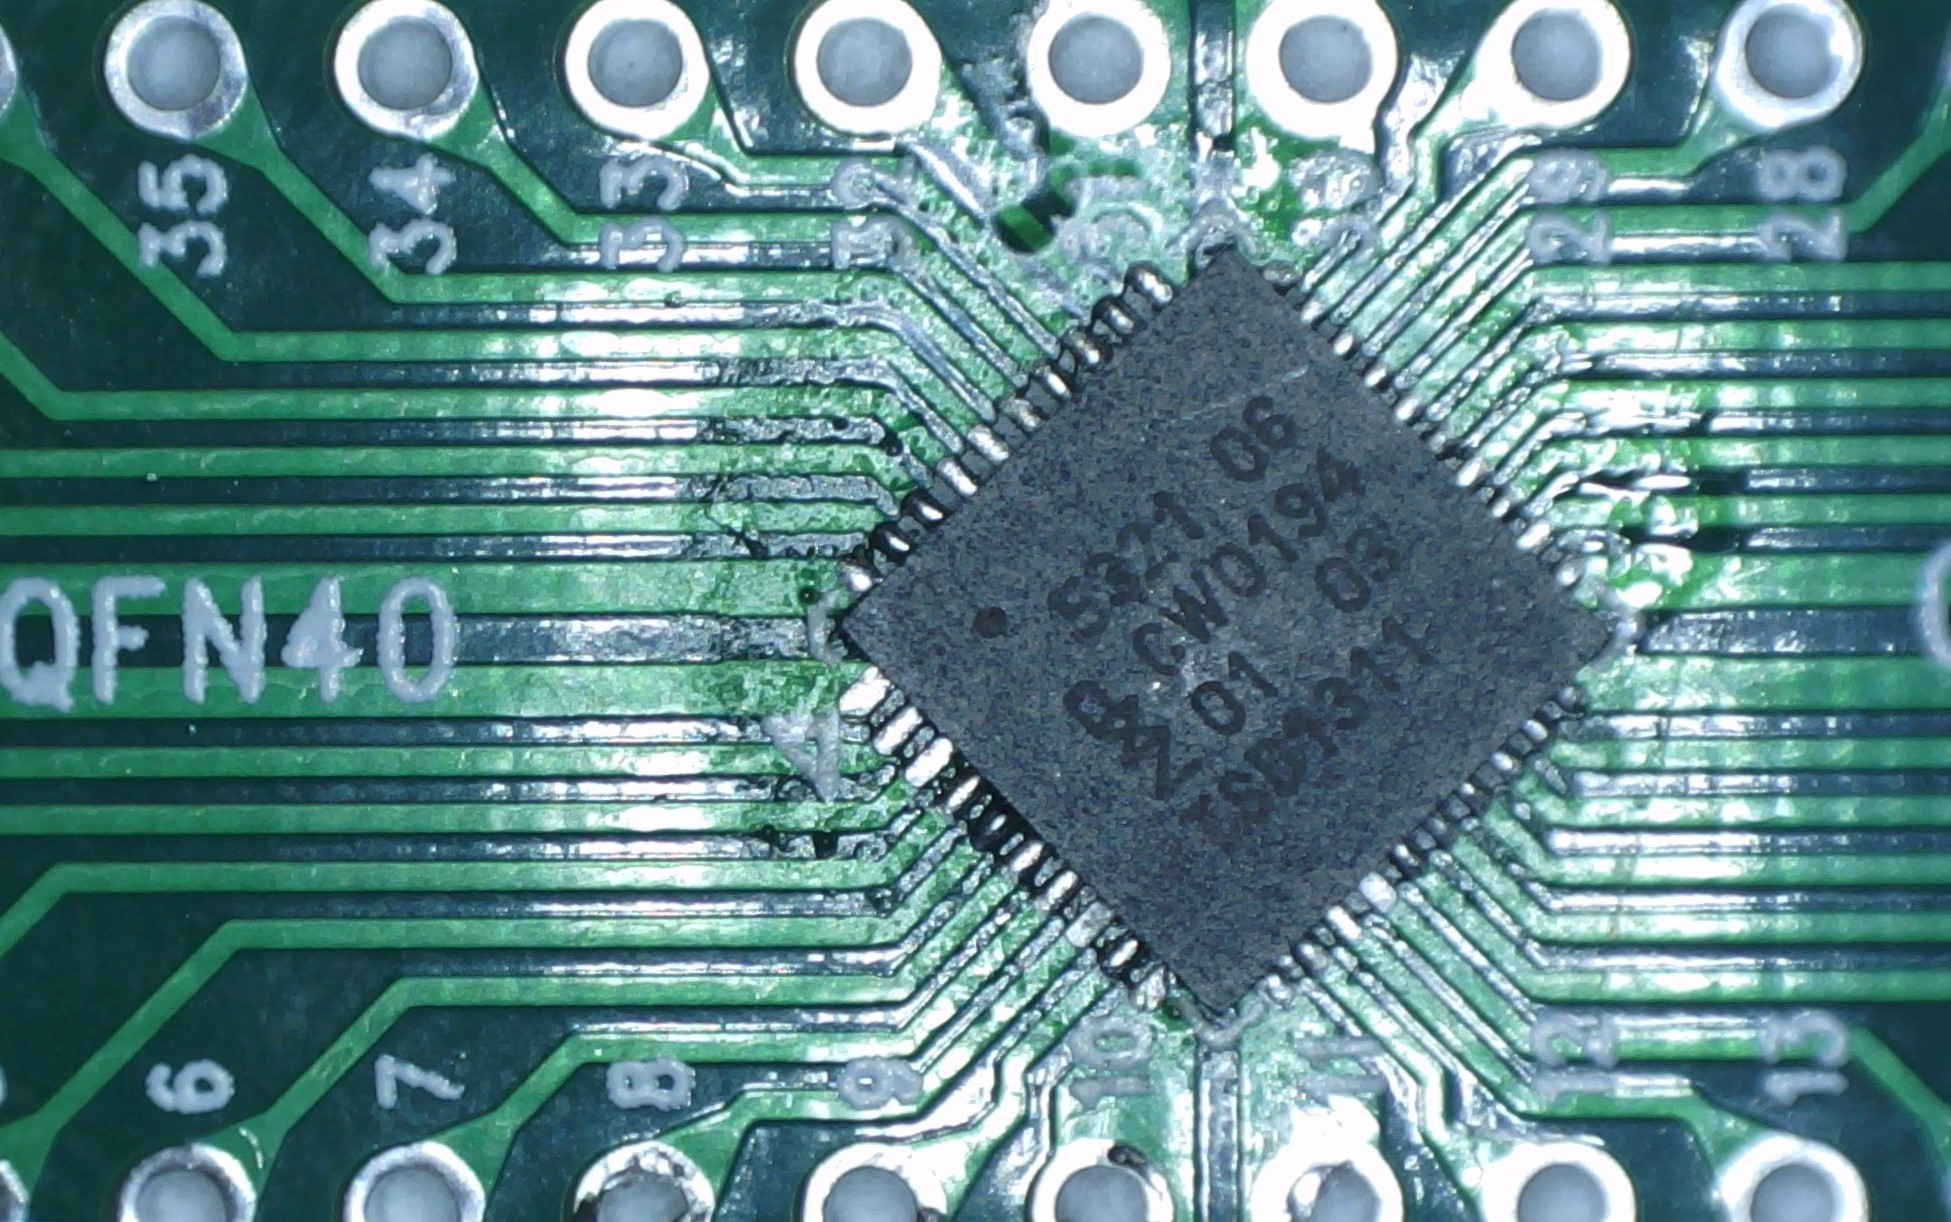
\includegraphics[scale = 0.15]{PN532}
		}
		\end{center}
		\caption{PN532}
	\end{figure}

    Since the processor translate messages of two protocol, one is from PN532 data sheet and the other is the protocol we design. Besides of strong processing ability, it also need some GPIO to control the coil selection and power on-off. For better performance and fewest foots, we use decoder such as 74HC138 to minimize foot use and use latch to control power. We have STC15W4K48S, QFP44 package, up to 33MHz 1T 8051 micro-controller.

\subsection{This is subsection}

    We have several advantages in providing a platform for IoT devices to work elegantly and efficiently, and probably to unify on-table devices with its manipulating mode, in a rather low cost and low complexity.
    
	\subsubsection{this is subsubsection}


\section{Paper Reading}

	\subsection{Intensive}
		\cite{SWless}
		\cite{SurNfc}
		\cite{WTraMag}
		\cite{magP}
		\cite{pocketC}
		\cite{wirelessALL}
	\subsection{extensive}
        \cite{6176332}
        \cite{6838830}
        \cite{7056164}
        \cite{6902086}
        \cite{Fei:2013:PPP:2512349.2514593}
        \cite{7428884}
        \cite{4782856}
	
{\small
	\bibliographystyle{ieee}
	\bibliography{SGbib}
}

\end{document}
